\documentclass{beamer}

\usepackage{fontspec}
\usepackage{xeCJK}
\setCJKmainfont{DFFN_R3.TTC}
\XeTeXlinebreaklocale "zh"
\XeTeXlinebreakskip = 0pt plus 1pt
\linespread{1.3}
\allowdisplaybreaks

\newcommand{\weib}{\CJKfamily{weib}}
\newcommand{\hkss}{\CJKfamily{hkss}}
\newcommand{\hksy}{\CJKfamily{hksy}}
\newcommand{\lth}{\CJKfamily{lth}}
\usepackage{color}
\usepackage{booktabs}
\usepackage{tabularx}
\usepackage{caption}
\usepackage{tikz}
\usepackage{verbatim}
\usepackage{pgfplotstable}
\pgfplotsset{width=12cm}
\pgfplotsset{height=7cm}
\pgfplotsset{compat=1.13}

\usetheme{EastLansing}
\usetikzlibrary{positioning}
\useinnertheme{rectangles}
\usefonttheme{professionalfonts}

\newcommand{\lw}{0.8mm}
\setbeamercovered{transparent}


%\AtBeginSection[]
%{
  %\begin{frame}<beamer>
	%\frametitle{報告大綱}
	%%\frametitle{RoadMap}
    %\tableofcontents[currentsection]
  %\end{frame}
%}

\title{Paper Report}
\subtitle{\textcolor[rgb]{0.00,0.50,1.00}{{Speech Processing \& Machine Learning Laboratory}}}
\author{徐瑞陽}
\date{2019/04/10}
\begin{document}



\begin{frame}
\maketitle
\end{frame}

\begin{frame}
  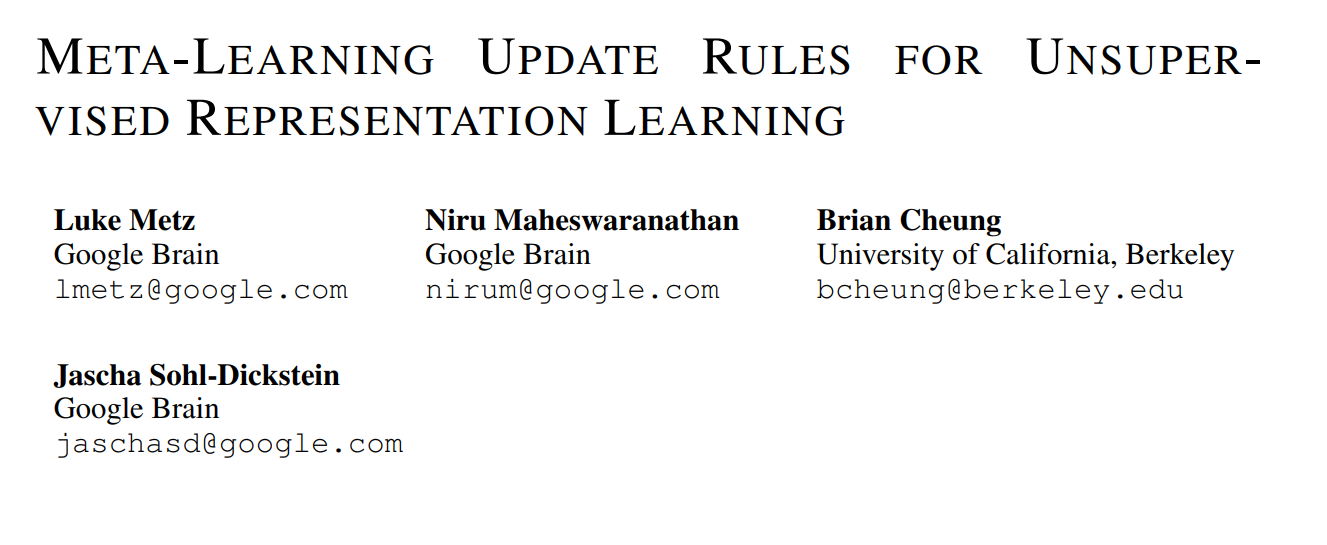
\includegraphics[width=\textwidth]{fig/title.png}
  \center ICLR 2019
  \center (8,8,8)
\end{frame}


\begin{frame}
\frametitle{Outline}
\tableofcontents
\end{frame}

\section{Survey on Meta Learning}
\begin{frame}
	\begin{center}
    %\weib{\LARGE{謝謝聆聽!}}
    \LARGE{Meta Learning}
	\end{center}
\end{frame}
\subsection{Problem Formulation}
\begin{frame}{Goal}

\[ \theta^\star = \arg \max_\theta \mathbb{E}_{\mathcal{D} \sim p(\mathcal{D}) }[\mathcal{A}_\theta(\mathcal{D})]\]

$\mathcal{A}$ depends on which application we want to learn \\ 
(e.g classification, regression... and MORE!!)
\end{frame}

\begin{frame}{One Instance - Few-shot classification}

  \[ \theta^\star = \arg \max_\theta \mathbb{E}_{L \subset \mathcal{L}} \, [ \mathbb{E}_{S^L \subset \mathcal{D}, B^L \subset \mathcal{D}}[\sum_{(x,y) \in B^L} \log P_\theta(y|x,S^L)] \,  ]\]

  \begin{itemize}
    \item sample subset of label $L \subset \mathcal{L}$ to split \texttt{meta-train}, \texttt{meta-test}
    \item $S^L$ is training data in \texttt{meta-train}, also called \textit{support set}
    \item $B^L$ is testing data in \texttt{meta-train}
    \item $(S^L, B^L)$ is called \textit{task} in some literature
    \item In this case, $\mathcal{A}_\theta$ is $P_\theta(y|x)$
  \end{itemize}
\end{frame}

\subsection{Common Approaches}
\begin{frame}{Common Approaches}
  \begin{itemize}
    \item Metric-based
    \item Model-based
    \item \textbf{Optimization-based}: The paper reported today focus on
  \end{itemize}
\end{frame}

\begin{frame}{Metric-based Approach}
  Meta-learn \textbf{weight of feature encoder}
  \[ P_\theta (y|x,S) = \sum_{(x,x_i) \in S} k_\theta (x,x_i) y_i \]
  \begin{itemize}
    \item $k_\theta$ is kernel function to measure similarity
    %\item good feature encoder imply good $k_\theta$
    \item Implementation: via \textbf{model structure design}
      \begin{itemize}
        \item Conv. Siamse NN ($\rightarrow$ Relation Network)
        \item Matching Network
        \item Prototypical Network
      \end{itemize}
    \item As far as I know, limited application in classification only
  \end{itemize}
\end{frame}

\begin{frame}{Model-base Approach}
  Meta-learn \textbf{strategy of using $S$}
  \[ P_\theta(y|x,S) = f_\theta(x,S) \]
  \begin{itemize}
    \item Retrieve experiences learnt in support set to answer
    \item Implementation: via external memory (e.g NTM), fusing $S$ (e.g convolution)
    \begin{itemize}
      \item NTM-based: MANN (LRUA, surprise-based) thru r/w weights
      \item Temporal Convolution: SNAIL (pretty brutal... )
    \end{itemize}
\end{itemize}
\end{frame}

\begin{frame}{Optimization-based Approach}
  %Meta-learn optimizer, initial weight, hyper-param, \textbf{update rule}...
  Meta-learn \textbf{hyper-param} (e.g optimizer, initial weights...)
  \[ P_\theta(y|x,S) = f_{g_\theta(S)}(x) \]
  \begin{itemize}
    \item Implementation: via gradients 
      \begin{itemize}
        \item initial weight: MAML and its variant\\
          (PMAML, FOMAML $\rightarrow$ Reptile)
        \item optimizer: LSTM Meta-Learner
        \item update rule: Today's paper
      \end{itemize}
  \end{itemize}
\end{frame}

\subsection{Applications}

\begin{frame}{Applications}
  \begin{itemize}
    \item Few-Shot classification
    \item Reinforcement learning
    \item Generative modeling: NMT (EMNLP 2018), TTS (ICLR 2019)
    \item \textbf{Unsupervised representation learning}
  \end{itemize}
\end{frame}

\begin{frame}{Desirable Properties}
  Quote from Chelsea Finn's PhD thesis
  \begin{itemize}
    \item Expressive power to represent ``learning algorithm''
    \item Generalization power
    \item Ambuiguity modeling power: what \textbf{P}MAML did
  \end{itemize}
\end{frame}


\section{Meta-Learning Update Rules For Unsupervised Learning}
\begin{frame}
  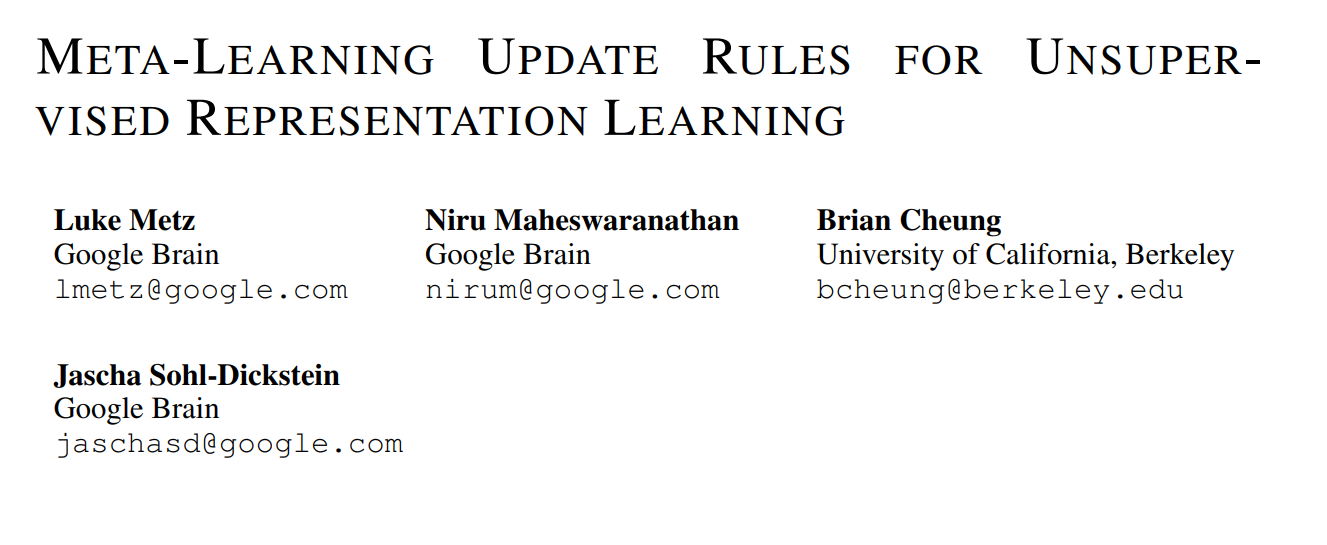
\includegraphics[width=\textwidth]{fig/title.png}
  \center ICLR 2019
\end{frame}

\begin{frame}{Motivation}
  \begin{itemize}
    \item Align objectives of unsupervised learning and human-specified downstream tasks
    \item Tackle this problem via meta-learn \textbf{update rule}
  \end{itemize}
\end{frame}

\begin{frame}{Flow}
  \center 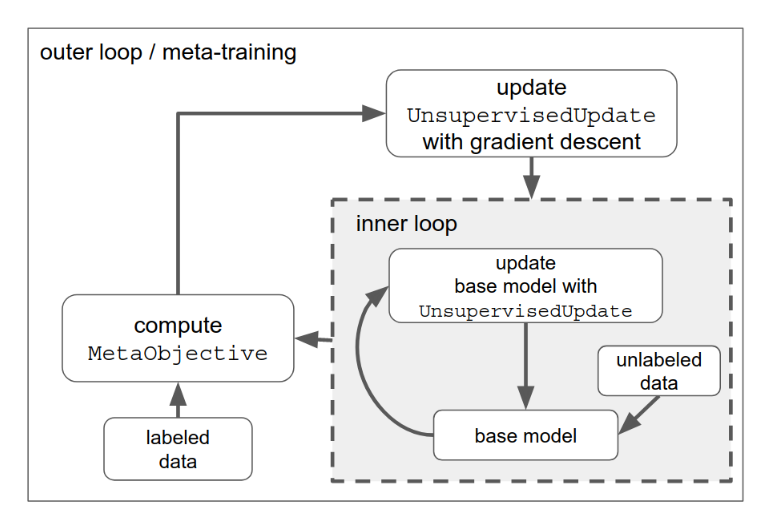
\includegraphics[width=0.7\textwidth]{fig/flow.png}
\end{frame}

\begin{frame}{Flow}
  \center 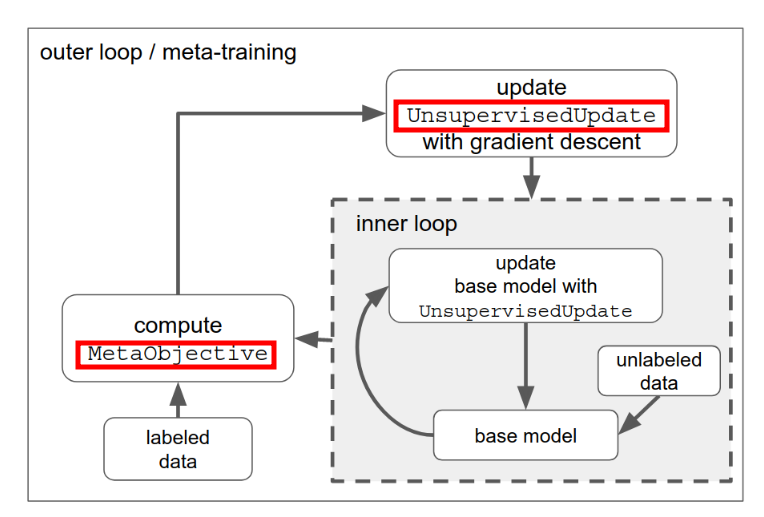
\includegraphics[width=0.7\textwidth]{fig/flow-anno.png}
  \begin{itemize}
    \item base model: $\text{MLP}_{\phi}$, acted as feature extractor (output is $x^L$)
  \end{itemize}
\end{frame}

\begin{frame}{Flow - Meta Objective}
  \begin{itemize}
    \item What to learn: Fitting linear regression to limited labeled data 
    \item Each task in \texttt{meta-train}: $\lbrace x_i \rbrace_{\text{unlabeled}}, \lbrace (x_a,y_a) \rbrace_\text{train}, \lbrace (x_b,y_b) \rbrace_\text{test}$
  \end{itemize}
  
  \begin{block}{Meta Objective}
    \[ \hat{v} = \arg \min_v (||y_a - v^Tx_a^L||^2 + \lambda ||v||^2) \]
    \[ \text{MetaObjective}(\phi) = \text{CosDist}(y_b,\hat{v}^Tx_b^L) \]
  \end{block}
  
\end{frame}

\begin{frame}{Flow - Learned Update Rule}
  Hightlight
  \begin{itemize}
    \item neuron-local, function of \textbf{pre-} and \textbf{post-} synaptic neurons
    \item defined for any base model structure
  \end{itemize}
  %Notation
  %\begin{itemize}
    %\item 
  %\end{itemize}
\end{frame}

\begin{frame}
  \center 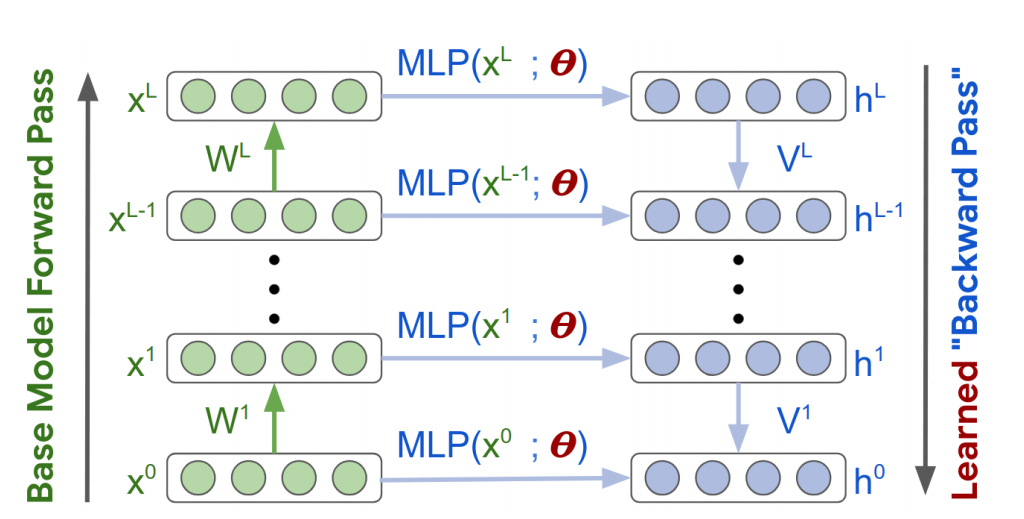
\includegraphics[width=0.7\textwidth]{fig/update-rule.png}
  \begin{itemize}
    \item base model $\phi = \lbrace W^1,b^1,V^1,\cdots,W^L,b^L,V^L \rbrace$
    \item $\triangle W_{ij}^L = \text{func}(h_i^l,h_j^{l-1}, W_{ij})$
    \item $h_i^l = \text{MLP}_\theta(x^l_i,z_i^l,V^{l+1},\delta^{l+1})$
    \item $z^l = \text{BatchNorm}(x^{l-1}W^l) + b^l$, $x^l = \text{ReLU}(z^l)$
    \item $\delta_i^l = \text{func}(h_i^l)$
  \end{itemize}
\end{frame}


\begin{frame}{Experiments - Preprocessing}
  \begin{itemize}
    \item Permute inputs along feature dimension (Note: same permutation in each task)
    \item \texttt{meta-train}: CIFAR10, ImageNet
    \item \texttt{meta-test}: MNIST, Fashion MNIST, \textbf{IMDB}
  \item \textbf{The paper haven't mention size of each task in experiments} \\
    (their source code can only run eval) (?)
  \end{itemize}
\end{frame}

\begin{frame}{Observations of Existing Representation Learning Algorithms}
  \begin{itemize}
    \item Objective function mismatch (e.g VAE)
    \item Need for consistent data structure (e.g ProtoNet)
  \end{itemize}
  \center 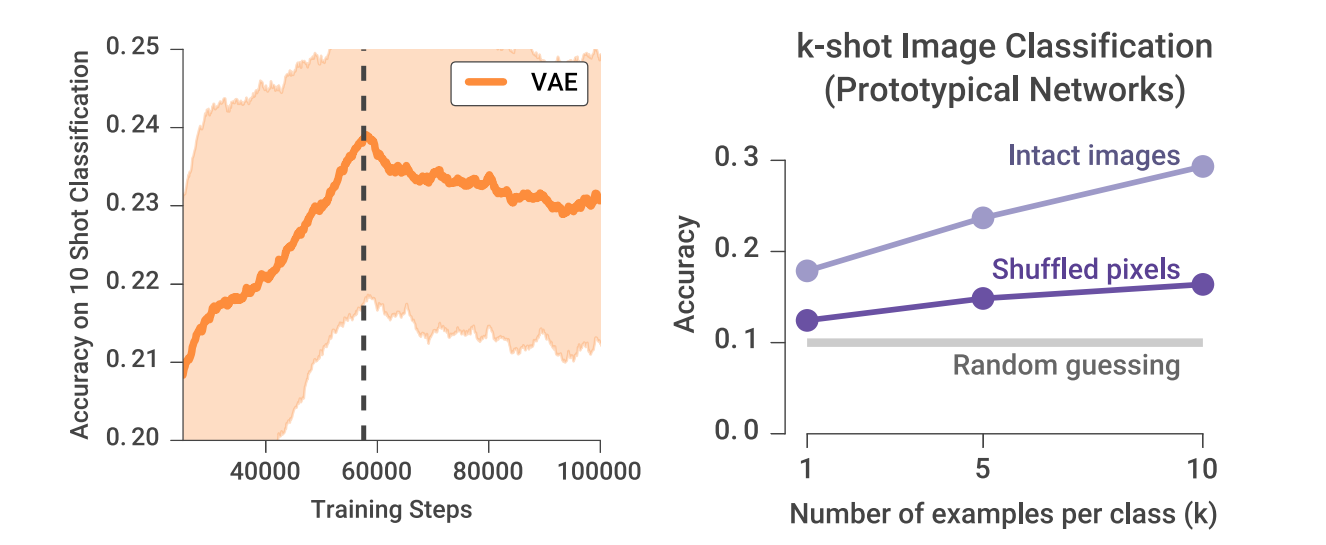
\includegraphics[width=\textwidth]{fig/obs.png}
\end{frame}

\begin{frame}{Generalization over datasets and domains}
  \center 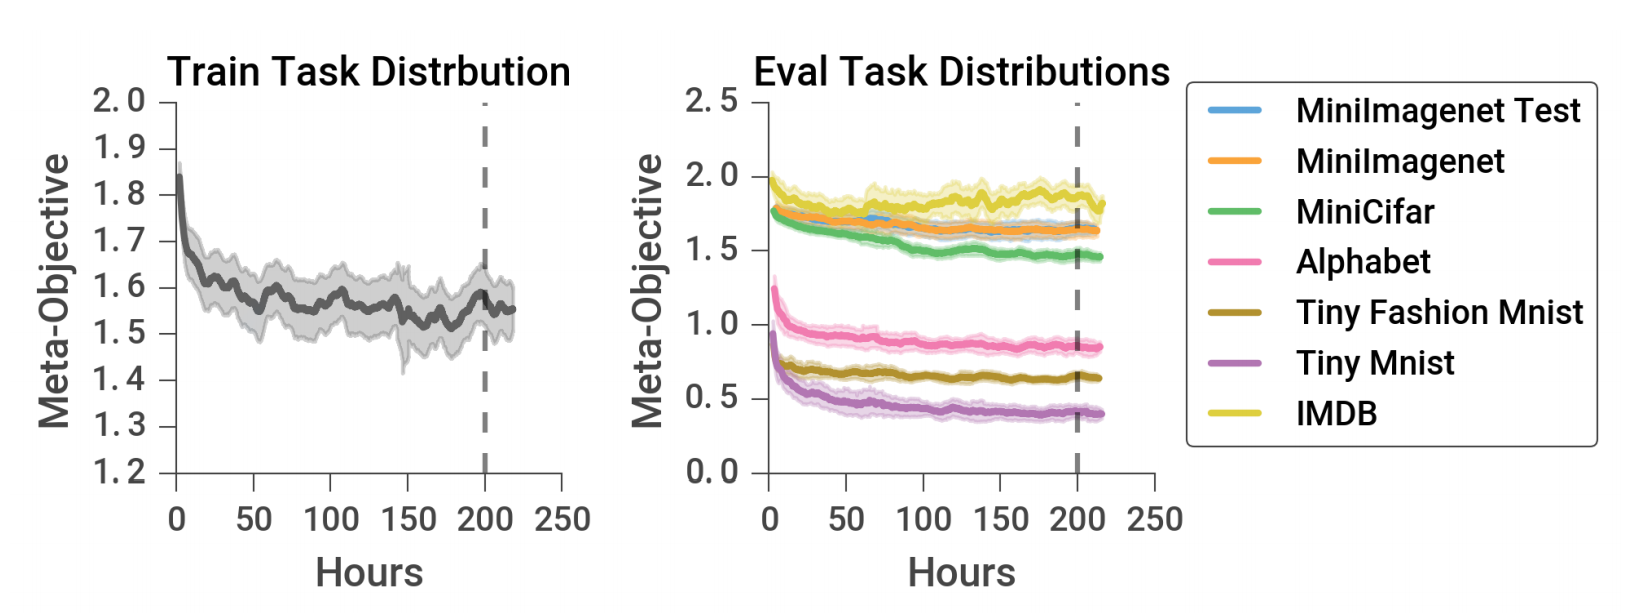
\includegraphics[width=\textwidth]{fig/lc.png}
\end{frame}

\begin{frame}{Generalization over datasets and domains}
  \center 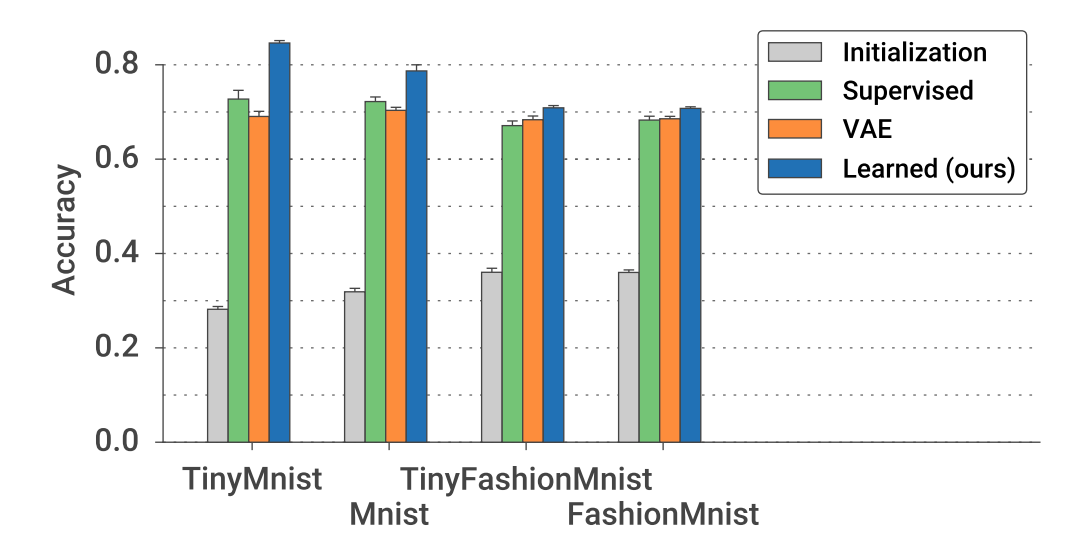
\includegraphics[width=\textwidth]{fig/mnist.png}
\end{frame}

\begin{frame}{Meta Overfitting}
  \center 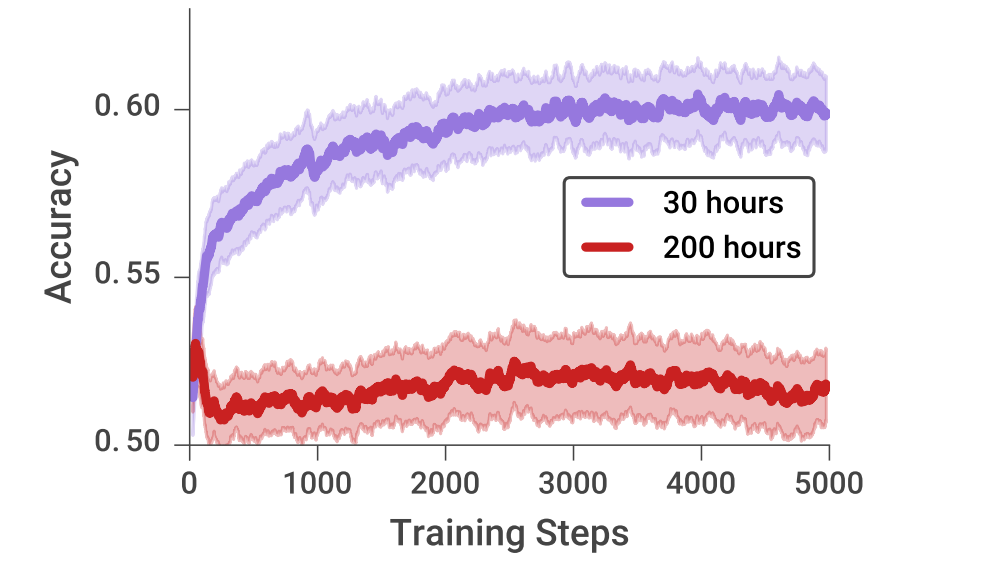
\includegraphics[width=0.7\textwidth]{fig/meta-overfitting.png}
  \begin{itemize}
    \item It seems that feature shuffling still cannot solve :p
  \end{itemize}
\end{frame}

\begin{frame}{Generalization over Network Architectures}
\end{frame}

\section{Comparison}
\subsection{Unsupervised Learning via Meta-Learning}

\begin{frame}
  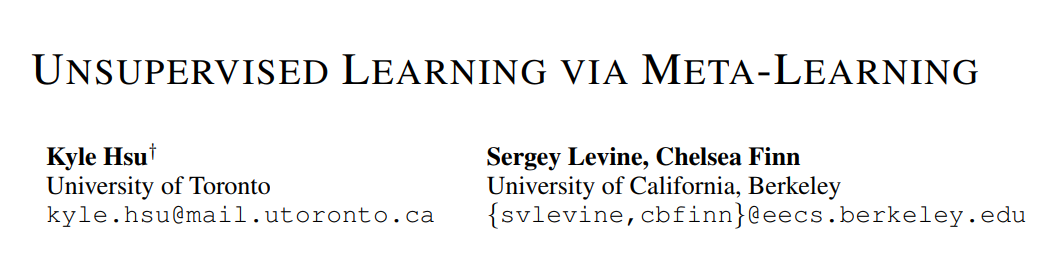
\includegraphics[width=\textwidth]{fig/ULML.png}
  \center ICLR 2019
\end{frame}

\begin{frame}
  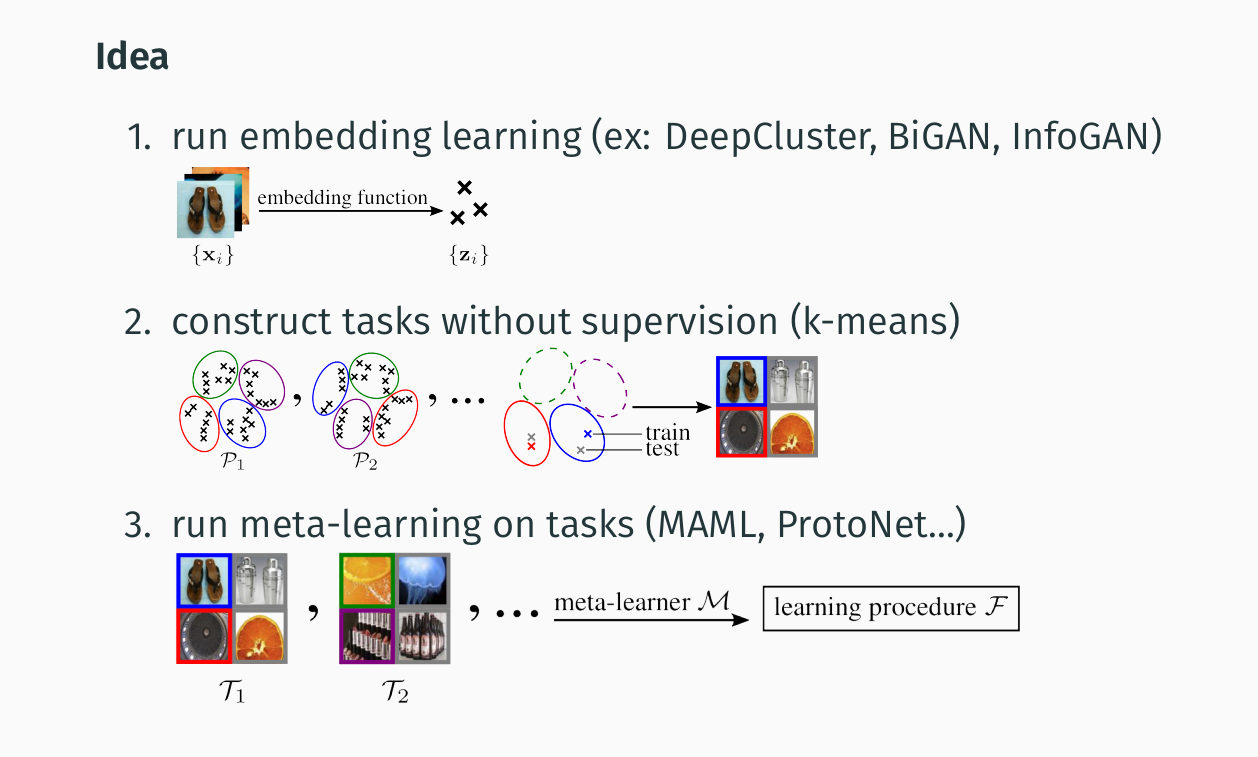
\includegraphics[width=\textwidth]{fig/ULML-flow.png}
  \textit{(source: 茅耀文's paper intro on 2019/01)}
\end{frame}

\begin{frame}{Difference}
  \begin{itemize}
    \item Assign labels through clustering (\textit{Automatic Task Construction}) as \texttt{meta-learn}
    %\item Meta-learn \textbf{parameters of embedding algorithm} // this is wrong!!
    %\item Learned representation has geometic semantics (depend on clustering)
    \item \textbf{Unsupervised Meta Learning} - since we didn't optimize the embedding algorithm actually\\
      (We use embedding $z \in \mathcal{Z}$ only because of its possible semantics which doesn't appear in raw input space $x \in \mathcal{X}$)
  \end{itemize}
  %\center \textbf{Unsupervised Meta Learning}\\
  %since we didn't optimize the embedding algorithm
\end{frame}

\subsection{LSTM Meta-Learner}
\begin{frame}
  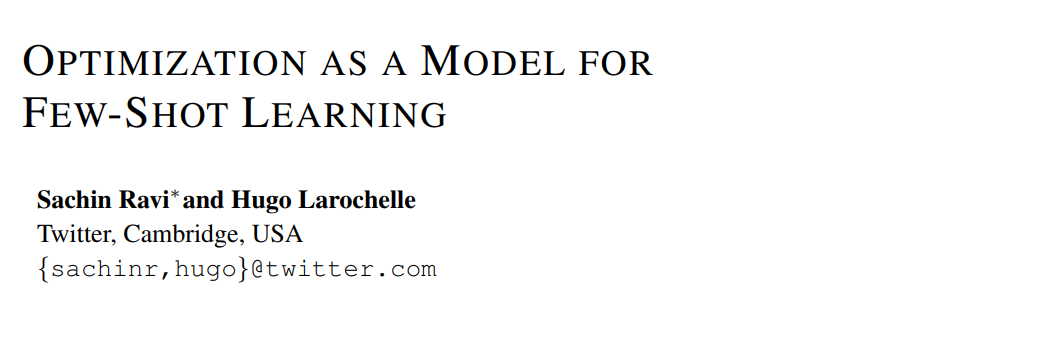
\includegraphics[width=\textwidth]{fig/LSTM-Meta-Learner.png}
  \center ICLR 2017
\end{frame}

\begin{frame}{Idea}
  \begin{itemize}
    \item SGD: $\theta_{t} = \theta_{t-1} - \alpha_t \nabla_{\theta_{t-1}} \mathcal{L}_t$
    \item LSTM update rule for cell state: $c_t = f_t \odot c_{t-1} + i_t \odot \tilde{c}_t$
    \item parametrize $i_t$ (and $f_t$) as meta-learner \\ 
      \quad \quad (function of $\nabla_{\theta_{t-1}}\mathcal{L}_t, \mathcal{L}_t, \theta_{t-1}, i_{t-1})$
  \end{itemize}
\end{frame}

\begin{frame}{Difference}
  \begin{itemize}
    \item It's similar actually, both of them meta-learn ``how to update param''
    \quad \quad Contribution of ``Meta-learn update rules'' is the proposed \textbf{unsupervised learning framework}
    \item Need to explicitly handle the magnitude difference of different params
  \end{itemize}
\end{frame}

\section{MISC}
\begin{frame}
	\begin{center}
    %\weib{\LARGE{謝謝聆聽!}}
    \LARGE{Questions?}
	\end{center}
\end{frame}


\subsection{Appendix}
\end{document} 
